% ============================================================================
% MÓDULO 1 — FUNDAMENTOS EPISTEMOLÓGICOS E CONCEITUAIS DA ANÁLISE AMBIENTAL
% CAPÍTULO 1 — A QUESTÃO AMBIENTAL CONTEMPORÂNEA E O PAPEL DA GEOGRAFIA
% ============================================================================

\aberturaModulo{MÓDULO 1}{FUNDAMENTOS EPISTEMOLÓGICOS E CONCEITUAIS}{Semanas 1 a 4 $\bullet$ Base dos Estudos Orientados EO1, EO2 e EO3 e Prova Teórica}{%
  Este módulo estabelece a base filosófica, histórica e conceitual do componente curricular \textbf{CHF662, Análise Ambiental}. Antes de aplicar matrizes de impacto, índices morfométricos de bacias hidrográficas ou técnicas de bioengenharia, o(a) geógrafo(a) precisa compreender \emph{por que} os problemas ambientais contemporâneos emergem, \emph{como} a relação sociedade--natureza foi historicamente construída e \emph{com que rigor} os conceitos centrais da área devem ser mobilizados.

  \vspace{6pt}
  \begin{itemize}[leftmargin=1.5em, itemsep=4pt]
    \item \textbf{Capítulo 1 (Semana 1):} \emph{A Questão Ambiental Contemporânea e o Papel da Geografia}, crise ambiental como crise civilizatória e de racionalidade (Leff, 2001), degradação dos solos, escassez hídrica e mudanças no uso da terra no Brasil e no Semiárido Baiano, crítica ao desenvolvimento sustentável (Porto-Gonçalves, 2006) e papel integrador da Geografia no planejamento ambiental.
    \item \textbf{Capítulo 2 (Semana 2, EO1):} \emph{A Modernidade, a Geografia e a Relação Sociedade--Natureza}, ruptura cartesiana, natureza como construção social (Porto-Gonçalves, 2006, p. 8--36), racionalidade instrumental, conflitos socioambientais na Bahia e no Nordeste e introdução à Geografia Socioambiental (Mendonça, 2001).
    \item \textbf{Capítulo 3 (Semana 3, EO2):} \emph{Abordagens Ambientais na Geografia e Análise Integrada}, consolidação da Geografia Socioambiental (Mendonça, 2001), articulação entre ambiente, território e paisagem (Bertrand, 2004) e superação da dicotomia físico--humano.
    \item \textbf{Capítulo 4 (Semana 4, EO3):} \emph{Conceitos e Definições Operacionais da Análise Ambiental}, distinção rigorosa entre ambiente, impacto ambiental, degradação, vulnerabilidade, fragilidade, risco, resiliência, recuperação e sustentabilidade (Sánchez, 2013; Tauk-Tornisielo, 1996).
    \item \textbf{Simulado do Módulo 1:} bateria integrada de verificação e treino dissertativo voltada à consolidação dos Estudos Orientados (EO1 a EO3) e à preparação progressiva para a Avaliação Teórica da Semana 10.
  \end{itemize}
}

\chapter{A Questão Ambiental Contemporânea e o Papel da Geografia}
\noindent\tagEmenta\par\vspace{6pt}

% ----------------------------------------------------------------------------
% ETAPA 1 — OBJETIVOS DE APRENDIZAGEM
% ----------------------------------------------------------------------------
\begin{capObjetivos}
Ao concluir este capítulo, você será capaz de:
\begin{enumerate}[leftmargin=1.6em, itemsep=2.5pt]
  \item Explicar por que a crise ambiental contemporânea configura uma crise civilizatória, de racionalidade e de conhecimento, e não apenas um conjunto isolado de falhas técnicas (Leff, 2001).
  \item Analisar a interação entre degradação dos solos, escassez hídrica e mudanças no uso da terra no contexto brasileiro, nordestino e do Semiárido Baiano, superando explicações estritamente climáticas ou deterministas.
  \item Diferenciar criticamente o discurso hegemônico de \emph{desenvolvimento sustentável} da perspectiva plural de \emph{sustentabilidade socioambiental} (Porto-Gonçalves, 2006; Leff, 2001).
  \item Distinguir abordagens disciplinares fragmentadas, multidisciplinares e interdisciplinares no diagnóstico e no planejamento ambiental.
  \item Fundamentar o papel integrador da Geografia na Análise Ambiental, conectando dinâmicas físico-bióticas e processos socioespaciais em múltiplas escalas.
\end{enumerate}
\end{capObjetivos}

% ----------------------------------------------------------------------------
% ETAPA 2 — REVISÃO DE PRÉ-REQUISITOS
% ----------------------------------------------------------------------------
\begin{capRevisao}
Antes de avançar na leitura teórica, retome quatro noções já trabalhadas nos semestres iniciais do Curso de Geografia:
\begin{itemize}[leftmargin=1.5em, itemsep=2.5pt]
  \item \textbf{Espaço geográfico:} conjunto indissociável de sistemas de objetos e sistemas de ações historicamente produzidos, no qual se materializam relações sociais, econômicas, políticas e naturais.
  \item \textbf{Ciclo hidrológico e cobertura vegetal:} a vegetação intercepta parte das chuvas, amortecendo o impacto das gotas sobre o solo, favorece a infiltração e reduz o escoamento superficial concentrado; sua remoção acelera a perda de solo e o assoreamento de corpos d'água.
  \item \textbf{Domínios morfoclimáticos e biomas da Bahia:} o território baiano abriga grande heterogeneidade ambiental, com destaque para a Caatinga (no domínio Semiárido, marcado por irregularidade pluviométrica e alta evapotranspiração), o Cerrado (no Oeste Baiano, importante zona de recarga de aquíferos) e remanescentes da Mata Atlântica (na faixa litorânea e no Recôncavo).
  \item \textbf{Escala geográfica:} todo fenômeno ambiental manifesta-se simultaneamente em escalas locais (uma encosta ou microbacia), regionais (um domínio semiárido ou bacia hidrográfica de grande porte) e globais (mudanças climáticas e cadeias de commodities).
\end{itemize}
\end{capRevisao}

% ----------------------------------------------------------------------------
% ETAPA 3 — EXPLICAÇÃO TEÓRICA
% ----------------------------------------------------------------------------
\etapa{3}{EXPLICAÇÃO TEÓRICA}

\begin{boxSimbolo}[Vocabulário Técnico e Conceitos-Chave do Capítulo]
\renewcommand{\arraystretch}{1.22}
\small
\begin{tabularx}{\textwidth}{@{}p{3.9cm} >{\raggedright\arraybackslash}X@{}}
  \toprule
  \textbf{Termo / Conceito} & \textbf{Definição Operacional em Análise Ambiental} \\
  \midrule
  \textbf{Questão ambiental} & Conjunto de tensões ecológicas, econômicas, políticas e culturais derivadas do modo como as sociedades contemporâneas se apropriam da natureza e distribuem benefícios e danos ambientais. \\
  \textbf{Crise civilizatória} & Crise estrutural do modelo moderno-industrial de produção, consumo e organização do conhecimento, cujos limites ultrapassam falhas pontuais de engenharia ou gestão (Leff, 2001). \\
  \textbf{Racionalidade econômica} & Lógica dominante voltada à maximização do crescimento, do lucro e da eficiência produtiva de curto prazo, frequentemente externalizando custos ecológicos e sociais. \\
  \textbf{Racionalidade ambiental} & Racionalidade alternativa orientada pela articulação entre produtividade ecológica, equidade social, diversidade cultural e gestão democrática do território (Leff, 2001). \\
  \textbf{Saber ambiental} & Campo emergente de conhecimentos que questiona a fragmentação científica tradicional e integra saberes disciplinares e locais em torno da complexidade socioambiental (Leff, 2001). \\
  \textbf{Interdisciplinaridade} & Rearticulação conceitual e metodológica entre diferentes áreas do conhecimento para responder a problemas complexos, indo além da mera soma de relatórios isolados. \\
  \textbf{Desenvolvimento sustentável} & Formulação institucional disseminada a partir do final do século XX que busca compatibilizar crescimento econômico, equidade social e conservação ambiental, frequentemente objeto de disputa política e crítica conceitual. \\
  \textbf{Sustentabilidade} & Condição socioecológica de manutenção dos processos vitais, da integridade dos ecossistemas e da reprodução digna das coletividades humanas no longo prazo (Porto-Gonçalves, 2006). \\
  \textbf{Planejamento ambiental} & Processo técnico, político e contínuo de diagnóstico, prognóstico, ordenamento de usos e definição de diretrizes voltadas à conservação, mitigação de impactos e recuperação de áreas degradadas. \\
  \bottomrule
\end{tabularx}
\end{boxSimbolo}

\section{A Questão Ambiental Contemporânea: Crise Civilizatória e de Racionalidade}

Na linguagem cotidiana e em parte da mídia, a expressão ``problema ambiental'' costuma aparecer reduzida a episódios visíveis e pontuais: um vazamento de óleo, o acúmulo de resíduos em um riacho urbano ou um incêndio florestal em determinado município. Embora esses eventos sejam graves e exijam resposta técnica imediata, reduzi-los a falhas isoladas impede a compreensão de suas causas estruturais.

A partir da segunda metade do século XX, especialmente após a aceleração industrial do pós-guerra, a intensificação da urbanização e a expansão globalizada das fronteiras agropecuárias e extrativistas, tornou-se evidente que os danos aos ecossistemas não eram acidentes marginais, mas consequências sistemáticas do próprio modelo de desenvolvimento adotado. É nesse horizonte que se consolida a \textbf{questão ambiental contemporânea}: um campo de debates científicos, políticos e territoriais que põe em xeque a forma como a sociedade moderna produz, consome, ocupa o espaço e constrói conhecimento.

Em \emph{Epistemologia ambiental} (2001, cap. 2: \emph{Interdisciplinaridade, ambiente e desenvolvimento sustentável}), Enrique Leff demonstra que a crise ambiental não é apenas uma crise ecológica (isto é, uma perturbação restrita aos ciclos biogeoquímicos), mas uma \textbf{crise civilizatória e de racionalidade}. Segundo o autor, a modernidade consolidou uma \textbf{racionalidade econômica e instrumental} que trata a natureza como estoque inesgotável de matérias-primas e como depósito passivo de rejeitos. Nessa lógica, os danos gerados sobre o solo, a água, a biodiversidade e a saúde humana são tratados como ``externalidades'', ficando de fora do cálculo econômico tradicional.

Ao mesmo tempo, essa racionalidade econômica apoiou-se na \textbf{fragmentação disciplinar do conhecimento científico}. Cada ciência especializou-se em recortar um fragmento da realidade: a agronomia focou a produtividade da cultura, a engenharia civil concentrou-se na resistência de estruturas, a economia modelou fluxos monetários e a sociologia examinou instituições humanas, muitas vezes sem diálogo efetivo entre si. Diante de fenômenos complexos como a desertificação, a degradação de bacias hidrográficas ou as mudanças climáticas, essa divisão estanque mostra-se insuficiente.

\begin{boxConceito}[Saber Ambiental e Interdisciplinaridade em Enrique Leff (2001)]
Para Leff (2001), superar a crise ambiental exige construir uma \textbf{racionalidade ambiental} sustentada por um \textbf{saber ambiental}. Esse saber não substitui o rigor de cada ciência, mas transforma internamente as disciplinas ao confrontá-las com os limites ecológicos e com a dimensão cultural e política do território. A \textbf{interdisciplinaridade ambiental}, portanto, não consiste em reunir especialistas para escrever capítulos separados em um mesmo relatório; trata-se de construir perguntas comuns, categorias integradoras e métodos articulados capazes de apreender o ambiente como totalidade complexa.
\end{boxConceito}

O esquema a seguir sintetiza a diferença estrutural entre a abordagem fragmentada, herdada da racionalidade econômica tradicional, e a abordagem integrada orientada pela racionalidade ambiental.

\begin{center}
\begin{tikzpicture}[
  node distance=0.55cm and 0.6cm,
  box/.style={draw=#1, fill=#1!8, rounded corners=3pt, line width=0.8pt, align=center, font=\footnotesize, inner sep=6pt, text width=4.4cm},
  head/.style={draw=#1, fill=#1, text=white, rounded corners=3pt, align=center, font=\footnotesize\bfseries, inner sep=5pt, text width=6.4cm},
  arr/.style={-{Stealth[length=2.2mm]}, line width=0.9pt, color=#1}
]
  % Coluna esquerda — Racionalidade Econômica
  \node[head=uefsAlert] (h1) at (0,0) {RACIONALIDADE ECONÔMICA / FRAGMENTADA};
  \node[box=uefsAlert, text width=6.4cm, below=0.35cm of h1] (e1) {\textbf{Concepção de natureza:} estoque passivo de insumos e receptor de rejeitos (externalidades).};
  \node[box=uefsAlert, text width=6.4cm, below=0.3cm of e1] (e2) {\textbf{Organização do saber:} disciplinas isoladas; diagnóstico fatiado por setor produtivo.};
  \node[box=uefsAlert, text width=6.4cm, below=0.3cm of e2] (e3) {\textbf{Consequência espacial:} respostas corretivas pontuais, persistência da degradação e conflitos.};
  \draw[arr=uefsAlert] (h1) -- (e1);
  \draw[arr=uefsAlert] (e1) -- (e2);
  \draw[arr=uefsAlert] (e2) -- (e3);

  % Coluna direita — Racionalidade Ambiental
  \node[head=uefsTeal] (h2) at (8.0,0) {RACIONALIDADE AMBIENTAL / INTEGRADA};
  \node[box=uefsTeal, text width=6.4cm, below=0.35cm of h2] (a1) {\textbf{Concepção de ambiente:} totalidade complexa e dinâmica entre sistemas físico-bióticos e sociedade.};
  \node[box=uefsTeal, text width=6.4cm, below=0.3cm of a1] (a2) {\textbf{Organização do saber:} interdisciplinaridade e diálogo entre ciência e saberes territoriais.};
  \node[box=uefsTeal, text width=6.4cm, below=0.3cm of a2] (a3) {\textbf{Consequência espacial:} planejamento preventivo, conservação, justiça socioambiental e gestão integrada.};
  \draw[arr=uefsTeal] (h2) -- (a1);
  \draw[arr=uefsTeal] (a1) -- (a2);
  \draw[arr=uefsTeal] (a2) -- (a3);

  % Seta de transição central
  \draw[arr=uefsGold, line width=1.4pt] (3.45,-2.35) -- node[above, font=\scriptsize\bfseries, color=uefsNavy, align=center]{Transição\\Epistemológica} (4.55,-2.35);
\end{tikzpicture}
\par\smallskip
{\small\color{uefsMuted}\textbf{Esquema 1.1:} Contraste entre racionalidade econômica fragmentada e racionalidade ambiental integrada (elaborado com base em Leff, 2001).}
\end{center}

Na prática da Análise Ambiental, é frequente confundir \emph{multidisciplinaridade} com \emph{interdisciplinaridade}. A Tabela~\ref{tab:disciplinas_cap1} apresenta os critérios operacionais que distinguem essas formas de organização do trabalho técnico e científico.

\begin{center}
\renewcommand{\arraystretch}{1.24}
\small
\begin{tabularx}{\textwidth}{@{}p{2.9cm} p{4.1cm} p{4.1cm} >{\raggedright\arraybackslash}X@{}}
  \toprule
  \rowcolor{uefsNavy}
  \textcolor{white}{\bfseries Dimensão} & \textcolor{white}{\bfseries Disciplinaridade Isolada} & \textcolor{white}{\bfseries Multidisciplinaridade} & \textcolor{white}{\bfseries Interdisciplinaridade Ambiental} \\
  \midrule
  \textbf{Formulação do problema} & Definida apenas nos limites de uma especialidade. & Cada área analisa o mesmo local sob sua própria ótica, em paralelo. & Problema construído conjuntamente, reconhecendo interações físico-bióticas e sociais. \\
  \rowcolor{bgGray}
  \textbf{Relação entre métodos} & Método único e fechado. & Justaposição de laudos e mapas que raramente dialogam entre si. & Integração metodológica (ex.: cruzamento entre uso da terra, erosão e vulnerabilidade social). \\
  \textbf{Produto típico} & Parecer setorial (ex.: apenas análise química da água). & Relatório ``colcha de retalhos'' com anexos desconectados. & Diagnóstico ambiental integrado com síntese causal e diretrizes coerentes de gestão. \\
  \rowcolor{bgGray}
  \textbf{Limite ou ganho} & Alta profundidade local, mas cegueira para causas sistêmicas. & Amplia o volume de dados, porém sem explicar as interações. & Permite intervir sobre as causas da degradação, e não apenas sobre seus sintomas. \\
  \bottomrule
\end{tabularx}
\par\smallskip
{\small\color{uefsMuted}\textbf{Tabela 1.1:} Comparação entre abordagens disciplinar, multidisciplinar e interdisciplinar na Análise Ambiental (elaborada com base em Leff, 2001; Tauk-Tornisielo, 1996).}\label{tab:disciplinas_cap1}
\end{center}

\section{Degradação dos Solos, Escassez Hídrica e Mudanças no Uso da Terra}

Para que o debate epistemológico não permaneça abstrato, é essencial observar como a crise ambiental se materializa na superfície terrestre. No Brasil, e de maneira particularmente aguda no Nordeste e no Semiárido Baiano, três processos interligados concentram grande parte dos desafios da Análise Ambiental: a \textbf{degradação dos solos}, a \textbf{escassez hídrica} e as \textbf{mudanças no uso e cobertura da terra}.

\subsection{Mudanças no Uso da Terra como Vetor Desencadeador}

A cobertura vegetal nativa exerce funções hidrogeomorfológicas decisivas: intercepta a precipitação, dissipa a energia cinética das gotas de chuva, fornece matéria orgânica que estabiliza os agregados do solo e mantém canais radiculares que ampliam a infiltração da água. Quando áreas de Caatinga, Cerrado ou Mata Atlântica são suprimidas sem planejamento conservacionista para dar lugar a pastagens extensivas de alta lotação, monocultivos mecanizados, abertura desordenada de estradas rurais, mineração ou expansão urbana em encostas e fundos de vale, altera-se abruptamente o balanço entre infiltração e escoamento superficial.

Na Bahia, esse processo assume expressões regionais distintas:
\begin{itemize}[leftmargin=1.5em, itemsep=2.5pt]
  \item \textbf{Semiárido Baiano (domínio da Caatinga):} combina supressão da vegetação lenhosa para extração de lenha e carvão, sobrepastoreio caprino/bovino em áreas já frágeis, manejo inadequado de lavouras de sequeiro e implantação de grandes infraestruturas (estradas, linhas de transmissão, parques energéticos) que expõem solos rasos e pedregosos (como Neossolos Litólicos e Planossolos) a chuvas concentradas em poucos meses do ano.
  \item \textbf{Oeste Baiano (domínio do Cerrado):} caracteriza-se pela rápida conversão de vegetação nativa em agricultura mecanizada de larga escala, intensificando a demanda por águas superficiais e subterrâneas e modificando a dinâmica de recarga em chapadões arenosos.
  \item \textbf{Faixa litorânea, Recôncavo e centros urbanos regionais (como o entorno de Feira de Santana):} evidencia impermeabilização acelerada do solo, supressão de áreas de preservação permanente (APPs) de nascentes, lagoas e riachos, lançamento de efluentes sem tratamento adequado e expansão de loteamentos sobre áreas sujeitas a alagamentos ou instabilidade de vertentes.
\end{itemize}

\begin{figure}[H]
  \centering
  \begin{minipage}[t]{0.48\textwidth}
    \centering
    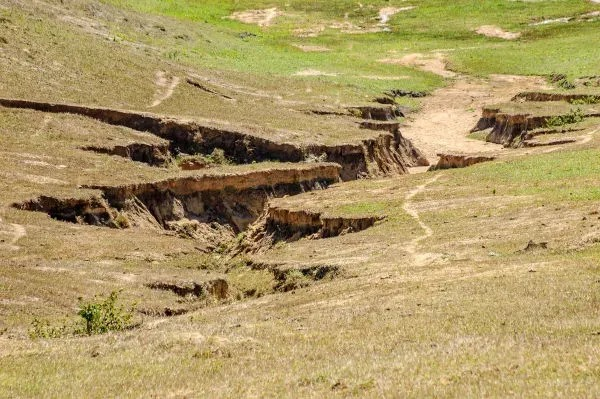
\includegraphics[width=\textwidth,height=4.4cm,keepaspectratio]{figures/foto_pastagem_ravinas.jpg}
    \par\small\textbf{(A)} Pastagem degradada com ravinas escalonadas e solo exposto.
  \end{minipage}\hfill
  \begin{minipage}[t]{0.48\textwidth}
    \centering
    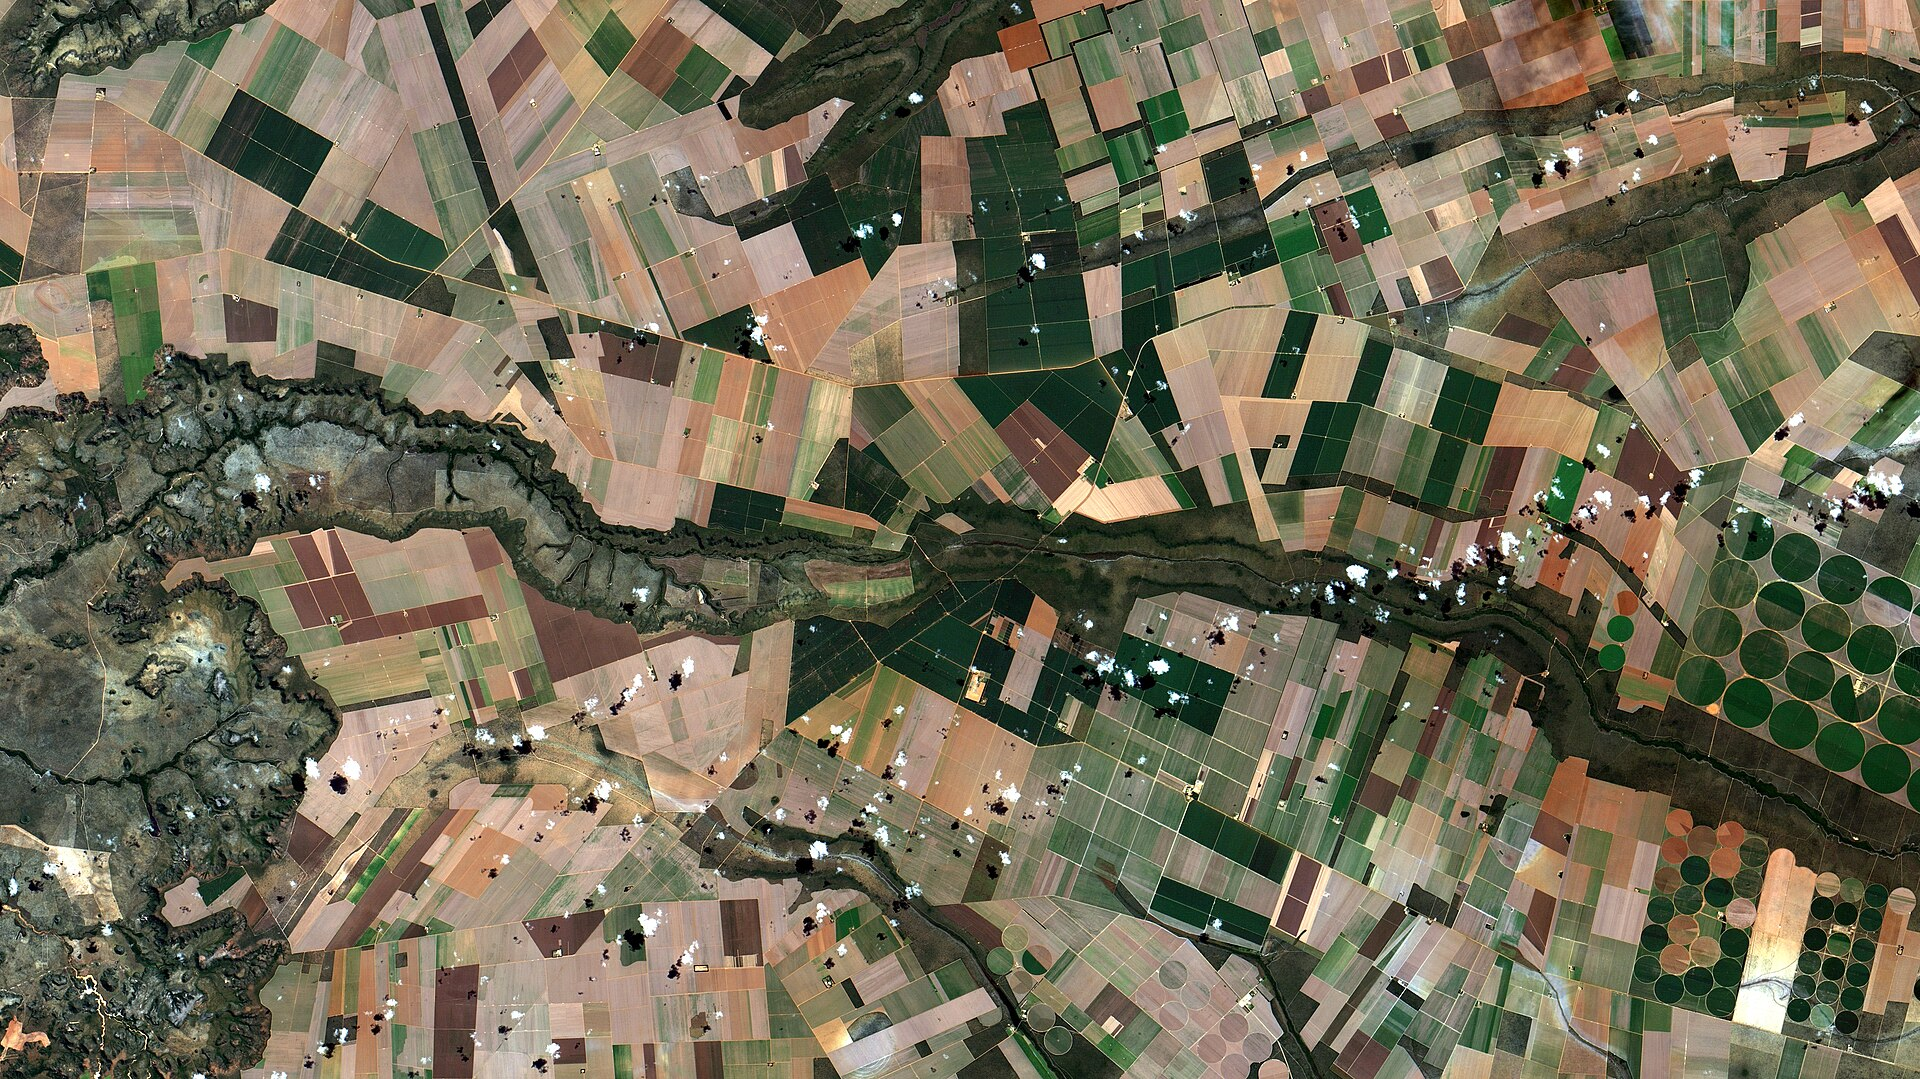
\includegraphics[width=\textwidth,height=4.4cm,keepaspectratio]{figures/foto_pivos_oeste_baiano.jpg}
    \par\small\textbf{(B)} Pivôs centrais de irrigação no Cerrado do Oeste Baiano (CBERS-4 MUX).
  \end{minipage}
  \caption{\textbf{Vetores de mudança no uso da terra na Bahia.} \textit{O que observar:} no painel A, a perda de cobertura vegetal em áreas de pastoreio intensivo expõe o solo ao escoamento concentrado e desencadeia incisões erosivas escalonadas. No painel B, os círculos escuros evidenciam a conversão em larga escala das chapadas do Oeste Baiano por agricultura irrigada mecanizada, elevando a pressão sobre a recarga hídrica. Fonte: Acervo didático CHF662 (A) e INPE/Wikimedia Commons, CC BY-SA (B).}
  \label{fig:vetores_bahia}
\end{figure}


\subsection{Degradação dos Solos e Processos Erosivos}

O solo não é um substrato inerte sobre o qual se constroem edificações ou se aplicam fertilizantes; trata-se de um corpo natural tridimensional, dinâmico e vivo, cuja formação (pedogênese) demanda séculos ou milênios. A degradação edáfica manifesta-se pela perda progressiva de suas funções físicas, químicas e biológicas: redução do teor de matéria orgânica, quebra dos agregados, selamento superficial, compactação pelo pisoteio animal ou tráfego de máquinas, salinização em perímetros irrigados mal drenados e remoção acelerada de partículas pela erosão hídrica e eólica.

Quando a taxa de remoção de solo supera amplamente a taxa natural de formação, a erosão evolui da forma \emph{laminar} (lavagem difusa da camada superficial mais fértil) para a forma \emph{linear} (sulcos, ravinas e voçorocas). Os sedimentos mobilizados das encostas não desaparecem: são transportados pela rede de drenagem e depositados em calhas fluviais, barreiros, cisternas rurais e açudes, reduzindo sua capacidade de armazenamento de água.

\subsection{Escassez Hídrica: Condição Climática versus Produção Socioambiental}

Um dos equívocos mais persistentes sobre o Nordeste brasileiro é explicar a escassez hídrica exclusivamente pela baixa média pluviométrica. O clima semiárido apresenta, de fato, chuvas concentradas no tempo, elevada variabilidade interanual e altas taxas de evapotranspiração potencial, características naturais que definem a \textbf{semiaridez}. Contudo, a \textbf{escassez hídrica vivenciada pela população} é resultado direto da interação entre essa dinâmica climática e fatores socioespaciais: desmatamento das cabeceiras e matas ciliares, compactação do solo (que impede a recarga do lençol freático), assoreamento de reservatórios, contaminação de mananciais e distribuição desigual da infraestrutura de captação e acesso à água.

\begin{boxConceito}[Cadeia de Retroalimentação Solo--Água--Uso da Terra]
  
Degradação dos solos, escassez hídrica e mudança no uso da terra não ocorrem como listas paralelas de problemas: elas formam um circuito retroalimentado. A supressão vegetal reduz a infiltração e intensifica o escoamento superficial; o escoamento acelerado remove o solo fértil e assoreia os corpos d'água; a perda de fertilidade e de disponibilidade hídrica pressiona os produtores a expandir o desmatamento sobre novas áreas frágeis, ampliando a vulnerabilidade socioambiental.
\end{boxConceito}

\begin{center}
\begin{tikzpicture}[
  node distance=0.45cm and 0.55cm,
  stepbox/.style={draw=uefsNavy, fill=bgSoft, rounded corners=3pt, line width=0.8pt, align=center, font=\footnotesize, inner sep=5pt, text width=3.2cm},
  alertbox/.style={draw=uefsAlert, fill=bgAlert, rounded corners=3pt, line width=0.9pt, align=center, font=\footnotesize, inner sep=5pt, text width=3.3cm},
  arr/.style={-{Stealth[length=2.2mm]}, line width=0.9pt, color=uefsNavy}
]
  \node[stepbox] (s1) at (0,0) {\textbf{1. Mudança no uso da terra}\\Supressão da Caatinga e sobrepastoreio};
  \node[stepbox] (s2) at (4.1,0) {\textbf{2. Degradação do solo}\\Exposição, selamento e menor infiltração};
  \node[stepbox] (s3) at (8.2,0) {\textbf{3. Dinâmica erosiva}\\Escoamento rápido, sulcos e ravinas};
  \node[alertbox] (s4) at (12.3,0) {\textbf{4. Escassez e risco}\\Assoreamento, menor recarga e vulnerabilidade};

  \draw[arr] (s1) -- (s2);
  \draw[arr] (s2) -- (s3);
  \draw[arr] (s3) -- (s4);

  % Seta de retroalimentação inferior
  \draw[arr, color=uefsAlert, dashed, line width=0.9pt] (s4.south) -- ++(0,-0.65) -| node[pos=0.25, below, font=\scriptsize\itshape, color=uefsAlert]{Retroalimentação positiva (ciclo amplificador): queda de produtividade pressiona novas áreas frágeis} (s1.south);
\end{tikzpicture}
\par\smallskip
{\small\color{uefsMuted}\textbf{Esquema 1.2:} Cadeia processual de retroalimentação entre uso da terra, degradação edáfica e escassez hídrica em ambientes semiáridos.}
\end{center}

\section{O Debate Crítico: Desenvolvimento Sustentável versus Sustentabilidade}

A partir da publicação do Relatório \emph{Nosso Futuro Comum} (Relatório Brundtland, 1987) e da Conferência das Nações Unidas sobre Meio Ambiente e Desenvolvimento (Rio-92), a expressão \textbf{desenvolvimento sustentável} ganhou enorme visibilidade internacional, sendo definida como aquele capaz de atender às necessidades do presente sem comprometer a capacidade das gerações futuras de atenderem às suas próprias necessidades.

À primeira vista, a formulação parece consensual e inquestionável. Entretanto, autores como Carlos Walter Porto-Gonçalves (\emph{Os (des)caminhos do meio ambiente}, 2006) e Enrique Leff (2001) demonstram que o conceito abriga contradições profundas. Porto-Gonçalves chama atenção para a estrutura política da expressão: ao acoplar o adjetivo ``sustentável'' ao substantivo ``desenvolvimento'', o discurso institucional dominante preserva intacto o projeto desenvolvimentista baseado na expansão contínua da produção de mercadorias, no consumo crescente de energia e na subordinação de territórios periféricos ao mercado mundial.

Sob essa perspectiva crítica, a noção de desenvolvimento sustentável muitas vezes opera como mecanismo de \emph{recodificação econômica da natureza}: a floresta, a água e o clima passam a ser valorados apenas como ``capital natural'' ou ``serviços mercantilizáveis'', sem questionar quem detém o controle dos territórios, quem se beneficia dos ganhos econômicos e quem arca com a poluição, o deslocamento compulsório e a degradação do solo.

Em contraposição, o debate sobre \textbf{sustentabilidade} (ou sustentabilidade socioambiental) propõe deslocar o foco do crescimento econômico ilimitado para a manutenção da integridade ecológica, da diversidade cultural e da equidade territorial. A sustentabilidade, nesse sentido, não é um selo de marketing empresarial nem uma meta técnica universalmente imposta de cima para baixo, mas um projeto histórico e geográfico que reconhece os limites biofísicos dos ecossistemas e valoriza modos locais de convivência com o ambiente, como as estratégias de convivência com o Semiárido baseadas em conservação de solo, captação descentralizada de água de chuva e manejo sustentável da Caatinga.

\begin{center}
\renewcommand{\arraystretch}{1.24}
\small
\begin{tabularx}{\textwidth}{@{}p{3.0cm} p{6.2cm} >{\raggedright\arraybackslash}X@{}}
  \toprule
  \rowcolor{uefsNavy}
  \textcolor{white}{\bfseries Critério de Análise} & \textcolor{white}{\bfseries Discurso Hegemônico de Desenvolvimento Sustentável} & \textcolor{white}{\bfseries Perspectiva Crítica de Sustentabilidade Socioambiental} \\
  \midrule
  \textbf{Eixo central} & Conciliar crescimento econômico contínuo com eficiência tecnológica e controle de impactos. & Garantir integridade dos sistemas ecológicos, justiça socioambiental e reprodução digna da vida. \\
  \rowcolor{bgGray}
  \textbf{Leitura da natureza} & Capital natural, estoque de recursos mensuráveis pelo mercado e ativos compensáveis. & Patrimônio socioecológico complexo, dotado de limites biofísicos e significados culturais plurais. \\
  \textbf{Papel da técnica} & Solução principal para a crise (ecoeficiência, substituição de insumos, mercado verde). & Ferramenta necessária, mas subordinada a critérios éticos, ecológicos e democráticos de decisão. \\
  \rowcolor{bgGray}
  \textbf{Relação com o território} & Tende a homogeneizar modelos produtivos e minimizar conflitos distributivos. & Reconhece conflitos territoriais, desigualdades de poder e diversidade de saberes locais. \\
  \textbf{Referência-base} & Crítica formulada em Leff (2001, cap. 2) e Porto-Gonçalves (2006). & Proposta articulada em Leff (2001), Porto-Gonçalves (2006) e na Geografia Socioambiental. \\
  \bottomrule
\end{tabularx}
\par\smallskip
{\small\color{uefsMuted}\textbf{Tabela 1.2:} Síntese comparativa entre o discurso convencional de desenvolvimento sustentável e a perspectiva crítica de sustentabilidade.}
\end{center}

\section{Planejamento Ambiental e o Papel Integrador da Geografia}

Diante de uma crise simultaneamente ecológica, econômica e territorial, o \textbf{planejamento ambiental} apresenta-se como instrumento fundamental de mediação entre a dinâmica da natureza e as demandas da sociedade. Planejar ambientalmente significa ir além de ações emergenciais pós-desastre: envolve levantar evidências empíricas sobre o meio físico, biótico e socioespacial (diagnóstico), projetar tendências de degradação ou recuperação sob diferentes cenários de uso da terra (prognóstico), estabelecer diretrizes de zoneamento, conservação e restauração (ordenamento) e acompanhar continuamente os resultados por meio de indicadores auditáveis (monitoramento).

É precisamente nesse terreno que a \textbf{Geografia} desempenha um papel integrador insubstituível frente à fragmentação disciplinar:
\begin{enumerate}[leftmargin=1.6em, itemsep=2.5pt]
  \item \textbf{Articulação físico-biótico--socioespacial:} a formação geográfica capacita o profissional a ler simultaneamente o relevo, os solos, a rede de drenagem e a cobertura vegetal juntamente com a estrutura fundiária, a urbanização, as redes de infraestrutura e os conflitos territoriais.
  \item \textbf{Domínio da espacialidade e da cartografia:} problemas ambientais nunca são abstratos; eles têm localização, extensão, conectividade e padrões espaciais que podem ser mapeados, modelados e cruzados em Sistemas de Informação Geográfica (SIG) e trabalhos de campo.
  \item \textbf{Leitura multiescalar:} o(a) geógrafo(a) conecta processos que ocorrem na escala da parcela de solo ou da vertente (erosão em sulcos) com a escala da bacia hidrográfica (assoreamento de mananciais), da região (políticas para o Semiárido) e das redes econômicas globais (demanda por energia e commodities).
  \item \textbf{Mediação interdisciplinar:} por transitar entre as ciências da Terra e as ciências humanas, a Geografia atua como ponte entre engenheiros, biólogos, agrônomos, gestores públicos e comunidades locais na construção de diagnósticos ambientais coerentes.
\end{enumerate}

\begin{boxDica}[Conexão Direta com os Próximos Módulos e o Trabalho Prático Final]
Tudo o que você estudará nos próximos capítulos de CHF662 desdobra os fundamentos apresentados aqui: no Módulo 2, a Avaliação de Impacto Ambiental (AIA) e a análise integrada; no Módulo 3, a bacia hidrográfica, a morfopedologia, os geossistemas e a fragilidade ambiental; no Módulo 4, os indicadores ambientais e de qualidade do solo (incluindo a viagem de campo no Semiárido Baiano); e no Módulo 5, a bioengenharia de água e solo, a legislação e o Diagnóstico Ambiental Aplicado (50\% da nota final). Manter desde o Capítulo 1 o hábito de integrar processos naturais e decisões sociais evitará diagnósticos fragmentados na Prova Teórica e no Trabalho Final.
\end{boxDica}

% ----------------------------------------------------------------------------
% ETAPA 4 — ESTUDOS DE CASO E EXEMPLOS RESOLVIDOS PASSO A PASSO
% ----------------------------------------------------------------------------
\etapa{4}{ESTUDOS DE CASO E EXEMPLOS RESOLVIDOS PASSO A PASSO}

\noindent\textit{Nota metodológica:} Os cenários numéricos e localidades estilizadas abaixo são \textbf{cenários didáticos ilustrativos}, construídos exclusivamente para treinar a aplicação rigorosa dos referenciais teóricos de Leff (2001) e Porto-Gonçalves (2006) a situações concretas da prática geográfica.

\begin{boxExemplo}{1.1: Básico}{Fragmentação Disciplinar em Projeto de Contenção de Erosão}
\passoEnunciado{Em um município fictício do Semiárido Baiano \textit{(cenário didático ilustrativo)}, uma prefeitura contratou uma empresa para conter o assoreamento de um açude comunitário. A equipe técnica elaborou apenas um projeto de dragagem mecânica do reservatório e construção de um muro de concreto próximo ao sangradouro, sem avaliar o uso do solo nas cabeceiras da microbacia nem ouvir os agricultores que utilizam a água. Dois anos após a obra, o açude voltou a apresentar acúmulo intenso de sedimentos.}
\passoDados{Intervenção exclusivamente estrutural/corretiva (dragagem e muro de concreto); ausência de diagnóstico da cobertura vegetal e dos solos nas vertentes a montante; ausência de participação dos usuários locais; retorno do assoreamento em 2 anos.}
\passoPedido{Diagnosticar a falha epistemológica e metodológica do projeto à luz de Enrique Leff (2001) e indicar como uma abordagem interdisciplinar geográfica reestruturaria a intervenção.}
\passoMetodo{Análise epistemológica baseada nos conceitos de \emph{racionalidade econômica/instrumental}, \emph{fragmentação disciplinar}, \emph{saber ambiental} e \emph{interdisciplinaridade} (Leff, 2001, cap. 2).}
\passoContas{%
  \begin{enumerate}[leftmargin=1.5em, itemsep=2pt]
    \item \textbf{Identificação do sintoma versus causa:} a dragagem atuou apenas sobre o sintoma final (sedimento acumulado no açude), ignorando a causa geradora nas vertentes a montante (solo exposto, erosão laminar e linear, retirada da vegetação ripária).
    \item \textbf{Diagnóstico epistemológico (Leff, 2001):} o projeto reproduziu a \emph{fragmentação disciplinar} e a \emph{racionalidade instrumental}, tratando um problema socioambiental complexo como mera questão pontual de engenharia civil.
    \item \textbf{Reestruturação interdisciplinar:} uma equipe coordenada sob perspectiva geográfica integrada deveria: (a) delimitar a microbacia de contribuição do açude; (b) mapear áreas de solo exposto, sobrepastoreio e focos erosivos nas cabeceiras; (c) dialogar com os agricultores para identificar pressões de uso da terra e saberes locais de manejo; e (d) combinar medidas conservacionistas na vertente (recomposição vegetal, retenção de enxurrada, manejo do pastoreio) com ações de manutenção do reservatório.
  \end{enumerate}
}
\passoResposta{O fracasso recorrente do projeto decorre da fragmentação disciplinar e da racionalidade instrumental, que trataram o assoreamento como falha pontual dissociada da dinâmica da microbacia e do uso social da terra. A solução exige abordagem interdisciplinar e planejamento integrado a montante e junto à comunidade.}
\passoVerificacao{A análise é ambientalmente coerente: dragar um açude sem reduzir a produção de sedimentos nas encostas apenas reinicia o ciclo de assoreamento a cada estação chuvosa, desperdiçando recursos públicos e mantendo a vulnerabilidade hídrica.}
\end{boxExemplo}

\begin{boxExemplo}{1.2: Básico}{Diferenciando Semiaridez Climática de Escassez Hídrica Socioambiental}
\passoEnunciado{Duas microbacias rurais vizinhas no Semiárido Baiano \textit{(cenário didático ilustrativo)} registram exatamente a mesma precipitação média anual de $580\text{ mm}$, concentrada entre novembro e março, sobre substrato geológico e relevo semelhantes. Na Microbacia A, $65\%$ da área mantém cobertura de Caatinga manejada, faixas de mata ciliar conservadas e práticas de retenção de água no solo; suas cacimbas permanecem com água na estação seca. Na Microbacia B, $78\%$ da área foi convertida em pastagem degradada com solo compactado e margens desmatadas; os reservatórios secam rapidamente após as chuvas e o solo apresenta sulcos erosivos.}
\passoDados{Precipitação idêntica ($580\text{ mm/ano}$) e substrato semelhante em ambas as microbacias. Microbacia A: $65\%$ de vegetação nativa, mata ciliar preservada, disponibilidade hídrica mantida na estiagem. Microbacia B: $78\%$ de pastagem degradada, solo compactado, margens desmatadas, rápida perda de água e erosão em sulcos.}
\passoPedido{Explicar por que o determinismo climático não explica a diferença observada entre as duas microbacias e demonstrar a relação causal entre uso da terra, solo e água.}
\passoMetodo{Análise comparativa controlada (mesmo clima, diferentes usos da terra) articulando processos hidrogeomorfológicos básicos e leitura socioambiental da escassez hídrica.}
\passoContas{%
  \begin{enumerate}[leftmargin=1.5em, itemsep=2pt]
    \item \textbf{Controle da variável climática:} como ambas as microbacias recebem $580\text{ mm/ano}$ sob o mesmo regime de chuvas concentradas, a diferença na disponibilidade de água na estação seca não pode ser atribuída apenas à falta de chuva.
    \item \textbf{Dinâmica na Microbacia A:} a cobertura vegetal protege a superfície do solo contra o impacto das gotas de chuva, mantém porosidade elevada e favorece a infiltração, recarregando o solo e os reservatórios rasos (cacimbas) para o período seco.
    \item \textbf{Dinâmica na Microbacia B:} a remoção da vegetação e a compactação reduzem a taxa de infiltração; assim, grande parcela dos $580\text{ mm}$ transforma-se rapidamente em escoamento superficial, gerando sulcos erosivos, arraste de sedimentos e baixa recarga hídrica subsuperficial.
    \item \textbf{Síntese conceitual:} a semiaridez é condição climática natural comum às duas áreas, mas a escassez hídrica severa na Microbacia B é agravada pelo modelo de uso e ocupação do solo.
  \end{enumerate}
}
\passoResposta{A diferença decorre do manejo do uso da terra e das condições do solo, e não apenas do clima: a degradação vegetal e edáfica na Microbacia B converte a chuva em escoamento rápido e erosão, reduzindo a infiltração e produzindo escassez hídrica socioambiental.}
\passoVerificacao{O raciocínio respeita o balanço hídrico elementar: para uma mesma entrada pluviométrica ($P = 580\text{ mm}$), quanto menor a infiltração em solos degradados, maior o escoamento superficial imediato e menor a água armazenada disponível durante a estiagem.}
\end{boxExemplo}

\begin{figure}[H]
  \centering
  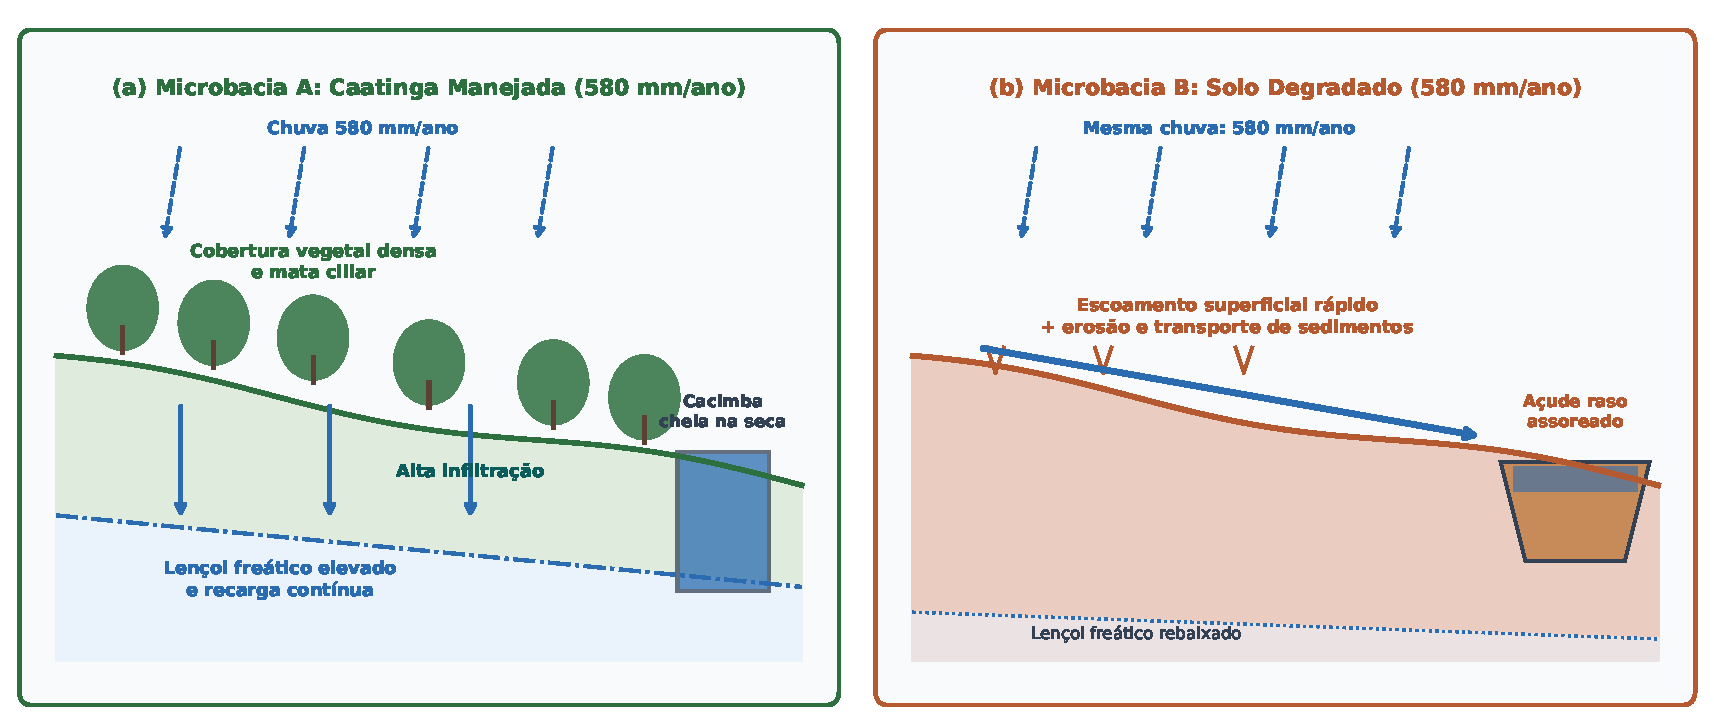
\includegraphics[width=0.96\textwidth]{figures/fig_cap01_contraste_microbacias.pdf}
  \caption{\textbf{Contraste hidrogeomorfológico entre semiaridez climática e escassez socioambiental.} \textit{O que observar:} sob a mesma precipitação anual de 580 mm, a Microbacia A conserva a cobertura arbustiva, favorece a infiltração e mantém o lençol freático elevado para abastecimento em cacimbas. Na Microbacia B, a compactação do solo redireciona a água para o escoamento superficial rápido, acelerando a erosão e o assoreamento do açude. Fonte: Elaboração didática CHF662.}
  \label{fig:contraste_microbacias}
\end{figure}


\begin{boxExemplo}{1.3: Intermediário}{Análise Crítica de um Discurso de ``Desenvolvimento Sustentável''}
\passoEnunciado{Um consórcio agroindustrial divulga um documento promocional anunciando a implantação de um polo de monocultura irrigada de exportação em uma bacia hidrográfica de transição Cerrado--Caatinga \textit{(cenário didático ilustrativo)}. O texto classifica o empreendimento como exemplo de ``desenvolvimento sustentável'' porque utilizará pivôs com sensores digitais que economizam $15\%$ de água em comparação a sistemas antigos e compensará a supressão de vegetação nativa mediante a compra de créditos ambientais em outra região do país.}
\passoDados{Alegações do consórcio: ganho de $15\%$ na eficiência de irrigação por sensores; compensação ambiental fora da bacia impactada; expansão de monocultura intensiva com remoção de vegetação nativa local e aumento da captação hídrica total.}
\passoPedido{Avaliar criticamente o uso do termo ``desenvolvimento sustentável'' nesse documento à luz de Porto-Gonçalves (2006) e Leff (2001), apontando as limitações socioambientais ocultadas pela peça promocional.}
\passoMetodo{Análise crítica do discurso ambiental com base na distinção entre \emph{desenvolvimento sustentável hegemônico} e \emph{sustentabilidade socioambiental} (Porto-Gonçalves, 2006; Leff, 2001).}
\passoContas{%
  \begin{enumerate}[leftmargin=1.5em, itemsep=2pt]
    \item \textbf{Análise do ganho de ecoeficiência ($15\%$):} economizar água por hectare em relação a técnicas antigas não garante redução do consumo total de água na bacia se a área irrigada se expandir de forma absoluta. A técnica melhora a eficiência produtiva sem questionar o limite hídrico regional.
    \item \textbf{Crítica à compensação desterritorializada:} comprar créditos ambientais em outra região trata a natureza como mercadoria intercambiável (lógica da racionalidade econômica criticada por Leff, 2001). Contudo, a biodiversidade, a proteção do solo e a recarga hídrica perdidas na bacia local não são fisicamente repostas por uma área conservada a centenas de quilômetros.
    \item \textbf{Ocultamento de dimensões sociais (Porto-Gonçalves, 2006):} o discurso adota o adjetivo ``sustentável'' para legitimar o modelo desenvolvimentista, omitindo questões centrais como quem perde acesso à água a jusante, como se alteram a estrutura fundiária e a segurança alimentar local e se as comunidades atingidas participaram da decisão.
  \end{enumerate}
}
\passoResposta{O documento emprega ``desenvolvimento sustentável'' em sentido retórico e mercadológico: reduz a questão ambiental à eficiência tecnológica parcial e à compensação financeira fora do território, desconsiderando limites hídricos da bacia e impactos socioespaciais locais.}
\passoVerificacao{A crítica é equilibrada e rigorosa: não nega a utilidade de sensores de irrigação, mas demonstra que eficiência técnica isolada não equivale à sustentabilidade ecológica e social em escala de bacia hidrográfica.}
\end{boxExemplo}

\begin{boxExemplo}{1.4: Intermediário}{Quantificação Didática de Mudanças no Uso da Terra em Microbacia}
\passoEnunciado{Durante um exercício de diagnóstico preliminar sobre uma microbacia fictícia de $1.200\text{ ha}$ no Semiárido Baiano \textit{(cenário didático ilustrativo)}, uma turma de Geografia comparou o mapeamento de uso e cobertura da terra entre dois anos de referência ($t_0$ e $t_1$, com intervalo de 15 anos) e obteve a tabela abaixo:}
\passoDados{%
  Área total da microbacia: $A_{\text{total}} = 1.200\text{ ha}$. Distribuição por classe:
  \begin{itemize}[leftmargin=1.5em, itemsep=1pt]
    \item Caatinga arbóreo-arbustiva densa: $660\text{ ha}$ em $t_0$ e $360\text{ ha}$ em $t_1$;
    \item Pastagem manejada e agricultura familiar diversificada: $300\text{ ha}$ em $t_0$ e $270\text{ ha}$ em $t_1$;
    \item Pastagem degradada com cobertura rala: $180\text{ ha}$ em $t_0$ e $390\text{ ha}$ em $t_1$;
    \item Solo exposto / áreas com erosão visível: $60\text{ ha}$ em $t_0$ e $180\text{ ha}$ em $t_1$.
  \end{itemize}
}
\passoPedido{(a) Calcular a variação absoluta (em $\text{ha}$), a variação relativa percentual de cada classe e a participação percentual das classes degradadas (pastagem degradada + solo exposto) em $t_0$ e $t_1$; (b) interpretar geograficamente o significado ambiental dessa trajetória.}
\passoMetodo{Cálculo passo a passo de variações absolutas ($\Delta A = A_{t_1} - A_{t_0}$), relativas ($\Delta\% = \frac{A_{t_1} - A_{t_0}}{A_{t_0}} \times 100\%$) e proporções sobre a área total ($p = \frac{A}{A_{\text{total}}} \times 100\%$), seguido de interpretação integrada solo--água--uso da terra.}
\passoContas{%
  \begin{enumerate}[leftmargin=1.5em, itemsep=2.5pt]
    \item \textbf{Conferência da área total:}
    Em $t_0$: $660 + 300 + 180 + 60 = 1.200\text{ ha}$.
    Em $t_1$: $360 + 270 + 390 + 180 = 1.200\text{ ha}$. (Conservação da área verificada.)

    \item \textbf{Variação absoluta ($\Delta A$) e relativa ($\Delta\%$) por classe:}
    \begin{itemize}[leftmargin=1.4em, itemsep=1.5pt]
      \item \emph{Caatinga densa:} $\Delta A = 360 - 660 = -300\text{ ha}$; $\Delta\% = \frac{-300}{660} \times 100\% \approx -45,5\%$.
      \item \emph{Pastagem manejada / agricultura familiar:} $\Delta A = 270 - 300 = -30\text{ ha}$; $\Delta\% = \frac{-30}{300} \times 100\% = -10,0\%$.
      \item \emph{Pastagem degradada:} $\Delta A = 390 - 180 = +210\text{ ha}$; $\Delta\% = \frac{+210}{180} \times 100\% \approx +116,7\%$.
      \item \emph{Solo exposto / erosão visível:} $\Delta A = 180 - 60 = +120\text{ ha}$; $\Delta\% = \frac{+120}{60} \times 100\% = +200,0\%$.
    \end{itemize}

    \item \textbf{Participação conjunta das classes degradadas sobre a área total:}
    \begin{itemize}[leftmargin=1.4em, itemsep=1.5pt]
      \item Em $t_0$: $A_{\text{deg},0} = 180 + 60 = 240\text{ ha} \implies p_0 = \frac{240}{1.200} \times 100\% = 20,0\%$.
      \item Em $t_1$: $A_{\text{deg},1} = 390 + 180 = 570\text{ ha} \implies p_1 = \frac{570}{1.200} \times 100\% = 47,5\%$.
      \item Acréscimo na participação degradada: $47,5\% - 20,0\% = +27,5\text{ pontos percentuais}$ (ou $+330\text{ ha}$).
    \end{itemize}

    \item \textbf{Interpretação geográfica integrada:} em 15 anos, a microbacia perdeu $45,5\%$ de sua cobertura nativa densa, enquanto a área de solo exposto triplicou ($+200\%$). Em $t_1$, quase metade da microbacia ($47,5\%$) encontra-se sob cobertura rala ou sem proteção vegetal, indicando elevada exposição à erosão hídrica, provável redução da infiltração, aceleração do escoamento superficial e risco crescente de assoreamento dos corpos d'água e queda de renda rural.
  \end{enumerate}
}
\passoResposta{A Caatinga densa retraiu $-300\text{ ha}$ ($-45,5\%$), o solo exposto triplicou ($+120\text{ ha}$; $+200,0\%$) e as classes degradadas saltaram de $20,0\%$ para $47,5\%$ da microbacia, configurando um quadro crítico de degradação hidrogeomorfológica e perda de sustentabilidade territorial.}
\passoVerificacao{Verificação aritmética e física: a soma das variações absolutas anula-se ($-300 - 30 + 210 + 120 = 0\text{ ha}$), confirmando consistência matemática; ambientalmente, o avanço de $27,5$ pontos percentuais de áreas degradadas justifica prioridade imediata de planejamento conservacionista e recuperação.}
\end{boxExemplo}

\begin{boxExemplo}{1.5: Avançado}{Diretrizes de Planejamento Ambiental Integrado em Área de Múltiplas Pressões}
\passoEnunciado{Na periferia de uma cidade média do interior da Bahia \textit{(cenário didático ilustrativo)}, uma bacia hidrográfica de pequeno porte concentra quatro processos simultâneos: (i) expansão de loteamentos populares sem drenagem pluvial em encostas de declividade moderada a forte; (ii) supressão da vegetação ciliar de um riacho intermitente que abastece hortas periurbanas; (iii) extração irregular de areia no leito do riacho para a construção civil; e (iv) lançamento de esgoto doméstico sem tratamento. A administração municipal propôs apenas ``multar os pequenos agricultores'' e ``canalizar o riacho com concreto''.}
\passoDados{Quatro vetores simultâneos de pressão (urbanização sem drenagem, desmatamento ciliar, mineração irregular de areia e esgoto doméstico) atuando na mesma microbacia; proposta municipal restrita a punição seletiva e canalização rígida.}
\passoPedido{Criticar a proposta municipal usando os conceitos de crise de racionalidade (Leff, 2001) e sustentabilidade crítica (Porto-Gonçalves, 2006) e formular quatro diretrizes integradas de planejamento ambiental lideradas por uma perspectiva geográfica.}
\passoMetodo{Integração dos referenciais epistemológicos do capítulo (Leff, 2001; Porto-Gonçalves, 2006) com os princípios do planejamento ambiental geográfico (diagnóstico multiescalar, interdisciplinaridade e participação social).}
\passoContas{%
  \begin{enumerate}[leftmargin=1.5em, itemsep=2.5pt]
    \item \textbf{Crítica à proposta municipal:}
    \begin{itemize}[leftmargin=1.4em, itemsep=1.5pt]
      \item \emph{Racionalidade instrumental:} canalizar o riacho com concreto transfere a velocidade do escoamento para jusante, agrava enchentes em outros trechos e elimina a função ecológica da calha natural, sem resolver o lançamento de esgoto nem a erosão das encostas.
      \item \emph{Injustiça socioambiental:} responsabilizar apenas os pequenos agricultores ignora a ausência de políticas habitacionais e de saneamento básico, bem como a cadeia econômica da construção civil que demanda areia ilegal.
    \end{itemize}
    \item \textbf{Quatro diretrizes integradas de planejamento ambiental:}
    \begin{itemize}[leftmargin=1.4em, itemsep=1.5pt]
      \item \emph{Diretriz 1, Diagnóstico espacial integrado da microbacia:} mapear uso da terra, áreas de risco nas encostas, pontos de lançamento de efluentes, cavas de extração mineral e trechos de APP degradada.
      \item \emph{Diretriz 2, Ordenamento territorial e saneamento:} disciplinar a expansão urbana, implantar drenagem sustentável (pavimentos permeáveis e bacias de retenção) e universalizar a coleta e o tratamento de esgoto.
      \item \emph{Diretriz 3, Recuperação hidrogeomorfológica e controle da extração:} coibir a lavra ilegal de areia com fiscalização e alternativas regulamentadas, recompor a mata ciliar e adotar técnicas conservacionistas nas vertentes.
      \item \emph{Diretriz 4, Gestão participativa e apoio à agricultura periurbana:} instituir comitê ou fórum da microbacia envolvendo moradores, horticultores, técnicos e poder público, convertendo os agricultores em agentes de conservação em vez de bodes expiatórios.
    \end{itemize}
  \end{enumerate}
}
\passoResposta{A proposta municipal fracassa por adotar solução tecnocrática e socialmente injusta; o planejamento ambiental geográfico exige diagnosticar os quatro vetores na escala da microbacia e articular ordenamento urbano, saneamento, recuperação ripária e gestão participativa.}
\passoVerificacao{As quatro diretrizes atacam simultaneamente os processos físicos (escoamento, erosão, qualidade da água) e as causas socioespaciais (habitação precária, déficit de saneamento, cadeia da construção civil), refletindo a passagem da fragmentação para a racionalidade ambiental.}
\end{boxExemplo}

% ----------------------------------------------------------------------------
% ETAPA 5 — ERROS CONCEITUAIS E METODOLÓGICOS MAIS COMUNS
% ----------------------------------------------------------------------------
\etapa{5}{ERROS CONCEITUAIS E METODOLÓGICOS MAIS COMUNS}

\begin{boxErro}[Erro 1.1: Reduzir a Crise Ambiental à ``Falta de Consciência Individual'']
\textbf{Equívoco frequente:} atribuir a degradação dos solos, a poluição hídrica ou o desmatamento exclusivamente à ``falta de educação'' ou a maus hábitos individuais dos cidadãos.

\textbf{Por que está incorreto:} embora práticas educativas sejam relevantes, esse argumento oculta determinantes estruturais (modelo econômico, padrão de uso da terra, concentração fundiária, déficit de saneamento e decisões políticas) que Leff (2001) identifica como núcleo da crise civilizatória.

\textbf{Como evitar:} analise sempre a articulação entre comportamentos locais, estruturas produtivas, políticas públicas e interesses econômicos em disputa no território.
\end{boxErro}

\begin{boxErro}[Erro 1.2: Confundir Multidisciplinaridade com Interdisciplinaridade Ambiental]
\textbf{Equívoco frequente:} acreditar que um estudo ambiental torna-se interdisciplinar apenas por conter capítulos separados escritos por um geólogo, um biólogo e um sociólogo.

\textbf{Por que está incorreto:} a mera justaposição de textos especializados sem diálogo metodológico caracteriza \emph{multidisciplinaridade}. Como mostra Leff (2001), a \emph{interdisciplinaridade ambiental} exige construir problemas integrados e explicar como processos físicos, bióticos e sociais condicionam-se mutuamente.

\textbf{Como evitar:} em seus relatórios e provas, explicite sempre as \emph{conexões causais} entre as variáveis (por exemplo, como uma decisão econômica de uso da terra altera a infiltração e agrava o assoreamento).
\end{boxErro}

\begin{boxErro}[Erro 1.3: Usar ``Desenvolvimento Sustentável'' como Sinônimo Neutro de ``Sustentabilidade'']
\textbf{Equívoco frequente:} empregar ambos os termos indistintamente, assumindo que qualquer projeto rotulado como ``desenvolvimento sustentável'' é ecologicamente íntegro e socialmente justo.

\textbf{Por que está incorreto:} conforme demonstra Porto-Gonçalves (2006), ``desenvolvimento sustentável'' é um conceito em disputa que frequentemente subordina a conservação ambiental à lógica do crescimento econômico contínuo e à mercantilização da natureza.

\textbf{Como evitar:} ao analisar políticas ou projetos, pergunte sempre: \emph{sustentável para quem, em qual escala espacial e com quais custos ecológicos e territoriais?}
\end{boxErro}

\begin{boxErro}[Erro 1.4: Explicar a Degradação do Semiárido pelo Determinismo Climático]
\textbf{Equívoco frequente:} afirmar que a erosão dos solos e a escassez hídrica no Semiárido Baiano são ``consequências inevitáveis da falta de chuva''.

\textbf{Por que está incorreto:} a semiaridez é uma condição climática natural à qual a Caatinga é evolutivamente adaptada. A degradação severa do solo e a vulnerabilidade hídrica resultam da combinação entre chuvas concentradas e práticas inadequadas de desmatamento, sobrepastoreio, compactação e desigualdade no acesso à água.

\textbf{Como evitar:} separe claramente o que é \emph{condicionante climático natural} do que é \emph{processo agravado pelo manejo e pela organização socioespacial}.
\end{boxErro}

% ----------------------------------------------------------------------------
% ETAPA 6 — EXERCÍCIOS DE FIXAÇÃO
% ----------------------------------------------------------------------------
\etapa{6}{EXERCÍCIOS DE FIXAÇÃO}

\subsection*{Nível 1: Básicos (Compreensão Conceitual)}

\begin{enumerate}[leftmargin=1.8em, itemsep=4pt]
  \item Explique, com base em Enrique Leff (2001), por que a crise ambiental contemporânea não pode ser compreendida apenas como uma crise ecológica ou tecnológica, mas como uma crise civilizatória e de racionalidade.
  \espacoResolucao[1.8cm]

  \item Diferencie \emph{racionalidade econômica} de \emph{racionalidade ambiental} segundo Leff (2001), indicando o papel das chamadas ``externalidades'' no primeiro caso.
  \espacoResolucao[1.8cm]

  \item Apresente duas diferenças fundamentais entre a abordagem \emph{multidisciplinar} e a abordagem \emph{interdisciplinar} na elaboração de diagnósticos ambientais.
  \espacoResolucao[1.8cm]

  \item Explique por que a supressão da vegetação nativa desencadeia simultaneamente processos de degradação do solo e alterações na disponibilidade hídrica de uma microbacia.
  \espacoResolucao[1.8cm]

  \item Sintetize a diferença entre \emph{semiaridez climática} e \emph{escassez hídrica socioambiental} no contexto do Semiárido Baiano.
  \espacoResolucao[1.8cm]

\subsection*{Nível 2: Intermediários (Análise Crítica e Aplicação)}

  \item Com base em Porto-Gonçalves (2006), analise criticamente a tensão existente entre o substantivo ``desenvolvimento'' e o adjetivo ``sustentável'' na expressão \emph{desenvolvimento sustentável}.
  \espacoResolucao[1.8cm]

  \item Um município baiano pretende elaborar um plano de conservação de nascentes, mas contratou estudos isolados de geologia, botânica e economia que não se comunicam entre si. Identifique o limite metodológico desse procedimento e proponha como a Geografia pode exercer papel integrador nesse planejamento ambiental.
  \espacoResolucao[1.8cm]

  \item Em um cenário didático ilustrativo, uma microbacia de $800\text{ ha}$ no Semiárido passou, em 10 anos, de $520\text{ ha}$ para $320\text{ ha}$ de cobertura nativa de Caatinga, enquanto a área de solo exposto cresceu de $40\text{ ha}$ para $140\text{ ha}$. Calcule a variação absoluta (em $\text{ha}$) e percentual de ambas as classes e explique dois desdobramentos esperados sobre o escoamento superficial e o assoreamento local.
  \espacoResolucao[1.8cm]

  \item Compare brevemente os principais vetores contemporâneos de mudança no uso da terra no Semiárido Baiano e no Oeste Baiano (Cerrado), destacando como a escala regional orienta o diagnóstico geográfico.
  \espacoResolucao[1.8cm]

  \item Por que a adoção exclusiva de soluções de ecoeficiência (como redução pontual de consumo de insumos por unidade produzida) pode ser insuficiente para alcançar a sustentabilidade socioambiental de um território? Relacione sua resposta a Leff (2001).
  \espacoResolucao[1.8cm]

\subsection*{Nível 3: Aplicados e Objetivos (Múltipla Escolha)}

  \item Segundo Enrique Leff (2001, cap. 2), a construção do \emph{saber ambiental} frente à crise contemporânea implica:
  \begin{alternativas}
    \item Substituir integralmente as ciências naturais por análises filosóficas, dispensando medições empíricas de solo e água.
    \item Somar relatórios independentes de diferentes áreas técnicas sem alterar os pressupostos de cada disciplina.
    \item Questionar a fragmentação do conhecimento e a racionalidade econômica hegemônica, rearticulando saberes disciplinares e locais sob uma racionalidade ambiental.
    \item Transferir a resolução dos impactos ambientais exclusivamente aos mecanismos automáticos de precificação do mercado financeiro.
    \item Restringir o debate ambiental à preservação de parques isolados, desvinculando-o do planejamento territorial e produtivo.
  \end{alternativas}
  \espacoResolucao[1.8cm]

  \item A respeito da cadeia de processos que conecta mudanças no uso da terra, degradação dos solos e escassez hídrica no Semiárido Baiano, assinale a alternativa \textbf{correta}:
  \begin{alternativas}
    \item A baixa infiltração de água no solo depende apenas da quantidade anual de chuvas, não sofrendo influência da cobertura vegetal ou da compactação.
    \item A retirada da vegetação nativa e o sobrepastoreio ampliam a exposição do solo, reduzem a infiltração, aceleram o escoamento superficial e intensificam a erosão e o assoreamento de reservatórios.
    \item A erosão laminar restringe-se a regiões tropicais úmidas de Mata Atlântica, não ocorrendo em áreas de Caatinga devido à baixa precipitação anual.
    \item O assoreamento de açudes é um processo benéfico no Semiárido porque aumenta a profundidade útil dos reservatórios na estação seca.
    \item A escassez hídrica nordestina decorre unicamente de anomalias climáticas naturais, sem relação com o desmatamento ciliar ou a gestão territorial.
  \end{alternativas}
  \espacoResolucao[1.8cm]

  \item Na leitura crítica proposta por Porto-Gonçalves (2006) sobre o conceito de \emph{desenvolvimento sustentável}, destaca-se que:
  \begin{alternativas}
    \item A expressão representa um consenso científico definitivo e neutro, aceito sem tensões políticas por todos os grupos sociais.
    \item O conceito rompe integralmente com a lógica de expansão contínua da produção de mercadorias adotada desde a Revolução Industrial.
    \item O adjetivo ``sustentável'' muitas vezes funciona como verniz legitimador do modelo desenvolvimentista hegemônico, ocultando desigualdades territoriais e limites ecológicos.
    \item A sustentabilidade só pode ser atingida mediante a homogeneização cultural e a substituição de saberes locais por pacotes tecnológicos globais.
    \item O debate sobre sustentabilidade restringe-se à gestão de resíduos sólidos urbanos, não abrangendo conflitos agrários ou hídricos.
  \end{alternativas}
  \espacoResolucao[1.8cm]

  \item Qual atributo caracteriza mais adequadamente o papel integrador da Geografia no planejamento ambiental frente à fragmentação disciplinar?
  \begin{alternativas}
    \item A capacidade de articular componentes físico-bióticos e processos socioespaciais em múltiplas escalas, empregando leitura espacial, trabalho de campo e mediação interdisciplinar.
    \item A exclusividade na realização de análises laboratoriais químicas de água e solo, dispensando a colaboração com outras áreas científicas.
    \item O foco exclusivo na descrição de aspectos fisiográficos naturais, deixando os fatores econômicos e políticos fora do diagnóstico ambiental.
    \item A padronização de soluções técnicas idênticas para qualquer região do país, independentemente das especificidades locais de relevo, clima e cultura.
    \item A substituição do diagnóstico empírico prévio por intervenções emergenciais de engenharia após a ocorrência de desastres ambientais.
  \end{alternativas}
  \espacoResolucao[1.8cm]

  \item Considere um cenário didático ilustrativo em que uma área rural teve $300\text{ ha}$ de vegetação nativa suprimidos em uma microbacia de $1.000\text{ ha}$ que originalmente possuía $600\text{ ha}$ de vegetação nativa. Sobre essa mudança no uso da terra, é \textbf{correto} afirmar que:
  \begin{alternativas}
    \item A vegetação nativa sofreu redução relativa de $30\%$ em relação à sua área inicial.
    \item A participação da vegetação nativa na microbacia passou de $60\%$ para $30\%$, representando perda relativa de $50\%$ da cobertura nativa original.
    \item A participação da vegetação nativa passou de $50\%$ para $20\%$ da área total da microbacia.
    \item A mudança no uso da terra não produz efeitos hidrológicos relevantes enquanto restar pelo menos $20\%$ de cobertura vegetal.
    \item A redução relativa da vegetação nativa foi de $60\%$, correspondendo à mesma taxa de aumento do volume de água armazenado no solo.
  \end{alternativas}
  \espacoResolucao[1.8cm]
\end{enumerate}

% ----------------------------------------------------------------------------
% ETAPA 7 — QUESTÕES DE PROVAS, ENADE E CONCURSOS AMBIENTAIS
% ----------------------------------------------------------------------------
\etapa{7}{QUESTÕES DE PROVAS, ENADE E CONCURSOS AMBIENTAIS}

\begin{enumerate}[leftmargin=1.8em, itemsep=5pt, start=16]
  \item \textbf{(Questão autoral, estilo ENADE / Concurso Ambiental)} Um relatório técnico estadual diagnosticou a degradação de uma bacia hidrográfica semiárida em três capítulos redigidos sem integração: o primeiro descreveu litologia e solos; o segundo listou espécies da flora; e o terceiro apresentou indicadores de renda municipal. Ao final, o documento atribuiu a escassez hídrica ``exclusivamente ao baixo índice pluviométrico da região'' e sugeriu a construção de barragens de concreto como única medida necessária. Com base nos fundamentos da Análise Ambiental (Leff, 2001; Porto-Gonçalves, 2006), avalie as afirmações a seguir:
  \begin{enumerate}[label=\Roman*., leftmargin=1.6em, itemsep=1.5pt]
    \item O relatório exemplifica uma abordagem multidisciplinar fragmentada, e não uma análise interdisciplinar integrada.
    \item A conclusão do relatório incorre em determinismo climático ao ignorar o papel do uso da terra, da cobertura vegetal e da desigualdade de acesso à água na produção da escassez hídrica.
    \item A recomendação exclusiva de obras de concreto expressa uma racionalidade instrumental que desconsidera a dinâmica das vertentes e os saberes locais de convivência com o Semiárido.
    \item A separação estanque entre capítulos físicos e socioeconômicos é o procedimento ideal na Geografia por garantir neutralidade científica.
  \end{enumerate}
  É correto apenas o que se afirma em:
  \begin{alternativas}
    \item I e IV.
    \item II e IV.
    \item I, II e III.
    \item II, III e IV.
    \item I, II, III e IV.
  \end{alternativas}
  \espacoResolucao[1.8cm]

  \item \textbf{(Questão autoral, estilo ENADE / Concurso Ambiental)} Para o cargo de Analista Ambiental em órgão público de gestão territorial, exige-se domínio conceitual das diferenças entre crescimento econômico, desenvolvimento sustentável e sustentabilidade socioambiental. Considerando a abordagem crítica trabalhada na Geografia contemporânea (Leff, 2001; Porto-Gonçalves, 2006), assinale a alternativa que expressa corretamente uma diretriz coerente com a \textbf{racionalidade ambiental}:
  \begin{alternativas}
    \item Aceitar a degradação severa de cabeceiras de drenagem em regiões semiáridas desde que compensada pela compra de títulos financeiros ambientais em outros biomas.
    \item Subordinar o zoneamento ambiental de uma bacia hidrográfica exclusivamente à taxa de retorno econômico de curto prazo dos empreendimentos licenciados.
    \item Priorizar o planejamento ambiental integrado em escala de bacia, articulando conservação do solo e da água, limites biofísicos dos ecossistemas, equidade social e participação das populações locais.
    \item Transferir a responsabilidade integral pela recuperação de áreas degradadas a campanhas pontuais de sensibilização individual, dispensando instrumentos de ordenamento territorial.
    \item Adotar pacotes tecnológicos uniformes em todos os biomas brasileiros, desconsiderando a diversidade ecológica da Caatinga, do Cerrado e da Mata Atlântica.
  \end{alternativas}
  \espacoResolucao[1.8cm]

  \item \textbf{(Questão autoral, estilo ENADE / Concurso Ambiental)} Ao planejar o diagnóstico ambiental de uma microbacia sujeita à conversão acelerada de vegetação nativa em pastagens extensivas, um(a) geógrafo(a) propõe relacionar o mapeamento multitemporal de uso da terra com o levantamento de focos erosivos, a situação das matas ciliares e as condições socioeconômicas dos produtores rurais. Essa proposta metodológica reflete:
  \begin{alternativas}
    \item Uma postura estritamente naturalista, pois privilegia processos geomorfológicos em detrimento da organização espacial humana.
    \item O papel integrador da Geografia na Análise Ambiental, ao articular variáveis físico-bióticas e socioespaciais para identificar causas sistêmicas da degradação e subsidiar o planejamento territorial.
    \item Um procedimento disciplinar isolado, uma vez que o uso de mapas multitemporais dispensa o diálogo com outras ciências ambientais.
    \item A aplicação direta da racionalidade econômica clássica, pois trata a perda de solo apenas como custo externo sem repercussão territorial.
    \item Uma limitação de escala, pois a análise de microbacias impede compreender conexões com dinâmicas regionais ou políticas públicas de conservação.
  \end{alternativas}
  \espacoResolucao[1.8cm]
\end{enumerate}

\begin{boxDica}[Orientações para o Estudo Orientado e a Prova Dissertativa (Semana 10)]
A Avaliação Teórica de CHF662 (Semana 10) tem caráter predominantemente dissertativo. Para responder com excelência às questões sobre o Capítulo 1, estruture seus textos em três passos:
\begin{enumerate}[leftmargin=1.5em, itemsep=2pt]
  \item \textbf{Ancoragem conceitual explícita:} cite e defina com precisão os autores e categorias da ementa, como \emph{crise civilizatória}, \emph{racionalidade ambiental} e \emph{interdisciplinaridade} em Leff (2001); crítica ao \emph{desenvolvimento sustentável} em Porto-Gonçalves (2006).
  \item \textbf{Cadeia causal físico-social:} demonstre como mudanças no uso da terra acionam degradação do solo e escassez hídrica, evitando respostas vagas ou deterministas.
  \item \textbf{Contextualização geográfica:} ilustre o argumento com realidades concretas da Bahia e do Semiárido, destacando a contribuição integradora da Geografia para o planejamento ambiental.
\end{enumerate}
\end{boxDica}

% ----------------------------------------------------------------------------
% ETAPA 8 — GABARITO COMENTADO (PÁGINA SEPARADA)
% ----------------------------------------------------------------------------
\clearpage
\etapa{8}{GABARITO COMENTADO}

\begin{boxGabarito}[Resolução Comentada: Nível 1 (Questões 1 a 5)]
\begin{enumerate}[leftmargin=1.8em, itemsep=4pt]
  \item \textbf{Crise civilizatória e de racionalidade (Leff, 2001):} Para Leff (2001), a crise ambiental revela os limites estruturais do projeto moderno-industrial de civilização. Ela decorre da forma como a sociedade organiza a produção (baseada no crescimento contínuo e na exploração ilimitada da natureza) e o próprio conhecimento (fragmentado em disciplinas isoladas). Por isso, ajustes puramente tecnológicos não bastam sem repensar a racionalidade que orienta a economia, a ciência e a relação com o ambiente.

  \item \textbf{Racionalidade econômica vs. racionalidade ambiental:} A \emph{racionalidade econômica} prioriza a maximização produtiva e financeira no curto prazo, tratando a degradação do solo, da água e da biodiversidade como ``externalidades'' fora do cálculo econômico. Já a \emph{racionalidade ambiental} busca reorientar a produção e o conhecimento com base na produtividade ecológica, na equidade social, na diversidade cultural e na sustentabilidade de longo prazo.

  \item \textbf{Multidisciplinaridade vs. interdisciplinaridade:} (i) Na \emph{multidisciplinaridade}, cada disciplina analisa o ambiente separadamente e justapõe resultados sem diálogo conceitual; na \emph{interdisciplinaridade}, o problema é formulado conjuntamente e os métodos são articulados para explicar interações causais. (ii) Enquanto a multidisciplinaridade tende a gerar diagnósticos fragmentados (``colchas de retalhos''), a interdisciplinaridade produz sínteses integradas capazes de orientar intervenções sobre as causas da degradação.

  \item \textbf{Supressão vegetal, solo e água:} Sem a proteção do dossel e da serapilheira, as gotas de chuva atingem o solo diretamente, desagregando partículas e causando selamento superficial. Isso reduz a infiltração da água (diminuindo a recarga do solo e dos aquíferos) e aumenta o escoamento superficial, que arrasta a camada fértil do solo, abre sulcos e ravinas e assoreia corpos d'água a jusante.

  \item \textbf{Semiaridez climática vs. escassez hídrica socioambiental:} A \emph{semiaridez} é uma característica climática natural definida pela irregularidade das chuvas e pela alta evapotranspiração. A \emph{escassez hídrica socioambiental}, por sua vez, é a falta de acesso seguro à água para consumo e produção, agravada pelo desmatamento de nascentes e matas ciliares, compactação dos solos, assoreamento de reservatórios e concentração desigual das infraestruturas hídricas.
\end{enumerate}
\end{boxGabarito}

\begin{boxGabarito}[Resolução Comentada: Nível 2 (Questões 6 a 10)]
\begin{enumerate}[leftmargin=1.8em, itemsep=4pt, start=6]
  \item \textbf{Tensão em ``desenvolvimento sustentável'' (Porto-Gonçalves, 2006):} O substantivo ``desenvolvimento'' carrega historicamente a lógica de expansão industrial, aumento do consumo energético e subordinação territorial ao mercado. Quando o adjetivo ``sustentável'' lhe é acrescentado sem alterar essa estrutura, o conceito tende a legitimar o mesmo modelo concentrador sob nova roupagem discursiva, ocultando conflitos sociais e limites biofísicos.

  \item \textbf{Limite metodológico e papel da Geografia:} O procedimento do município é apenas \emph{multidisciplinar} e fragmentado, incapaz de explicar como fatores geológicos, vegetais e econômicos interagem na degradação das nascentes. A Geografia integra esses elementos ao adotar recortes espaciais funcionais (como a microbacia hidrográfica), cruzar dados físico-bióticos e de uso da terra por meio de cartografia e campo, e articular o diagnóstico técnico às demandas das comunidades locais.

  \item \textbf{Cálculo e interpretação do cenário didático ($800\text{ ha}$):}
  \begin{itemize}[leftmargin=1.4em, itemsep=1.5pt]
    \item \emph{Caatinga nativa:} $\Delta A = 320 - 520 = -200\text{ ha}$; $\Delta\% = \frac{-200}{520} \times 100\% \approx -38,5\%$. (Em termos da área total, caiu de $65,0\%$ para $40,0\%$.)
    \item \emph{Solo exposto:} $\Delta A = 140 - 40 = +100\text{ ha}$; $\Delta\% = \frac{+100}{40} \times 100\% = +250,0\%$. (Em termos da área total, subiu de $5,0\%$ para $17,5\%$.)
    \item \emph{Desdobramentos esperados:} (1) elevação do escoamento superficial concentrado durante as chuvas intensas devido à menor infiltração nos $140\text{ ha}$ expostos; (2) maior transporte de sedimentos das vertentes para a rede de drenagem, acelerando o assoreamento de riachos e reservatórios locais.
  \end{itemize}

  \item \textbf{Vetores regionais na Bahia:} No \emph{Semiárido Baiano} (Caatinga), predominam pressões ligadas à supressão de vegetação lenhosa (lenha/carvão), sobrepastoreio extensivo, manejo inadequado de áreas frágeis e implantação de grandes infraestruturas sobre solos rasos. No \emph{Oeste Baiano} (Cerrado), sobressai a conversão mecanizada de grandes extensões de chapadões em monocultivos intensivos e irrigação em larga escala, pressionando a recarga hídrica regional. Reconhecer essa diferenciação regional evita diagnósticos genéricos e orienta estratégias adequadas a cada domínio.

  \item \textbf{Limites da ecoeficiência isolada (Leff, 2001):} Melhorar a eficiência técnica por unidade produzida não impede o aumento absoluto do consumo de solo, água e energia quando a escala de produção continua crescendo indefinidamente. Além disso, a ecoeficiência não resolve desigualdades territoriais nem conflitos pelo acesso aos recursos naturais, razão pela qual Leff (2001) defende a transição para uma racionalidade ambiental abrangente.
\end{enumerate}
\end{boxGabarito}

\begin{boxGabarito}[Resolução Comentada: Nível 3 e Questões de Provas/Concursos (Questões 11 a 18)]
\begin{enumerate}[leftmargin=1.8em, itemsep=4pt, start=11]
  \item \textbf{Gabarito: (C).} Leff (2001, cap. 2) define o saber ambiental como um campo que questiona a fragmentação disciplinar e a racionalidade econômica dominante, propondo a interdisciplinaridade e o diálogo com saberes locais. \emph{Incorretas:} (A) o saber ambiental não descarta medições empíricas das ciências naturais; (B) descreve multidisciplinaridade, não interdisciplinaridade; (D) o mercado não internaliza espontaneamente os limites ecológicos; (E) restringe a questão ambiental a áreas isoladas.

  \item \textbf{Gabarito: (B).} A remoção da vegetação nativa e o sobrepastoreio desprotegem e compactam o solo, reduzindo a infiltração, ampliando o escoamento superficial e intensificando erosão e assoreamento. \emph{Incorretas:} (A) a infiltração depende fortemente da vegetação e da estrutura do solo; (C) a erosão laminar é recorrente no Semiárido sob chuvas concentradas; (D) o assoreamento reduz, em vez de aumentar, a profundidade e o volume útil dos açudes; (E) reproduz o erro do determinismo climático.

  \item \textbf{Gabarito: (C).} Porto-Gonçalves (2006) mostra que o adjetivo ``sustentável'' frequentemente legitima o projeto desenvolvimentista tradicional sem alterar suas bases concentradoras e predatórias. \emph{Incorretas:} (A) trata-se de conceito em intensa disputa política; (B) o discurso convencional não rompe com a lógica de expansão contínua; (D) a sustentabilidade crítica valoriza a diversidade cultural e os saberes locais; (E) a temática abrange diretamente questões agrárias, hídricas e territoriais.

  \item \textbf{Gabarito: (A).} A força integradora da Geografia reside em articular componentes físico-bióticos e socioespaciais em múltiplas escalas, unindo leitura espacial, campo e mediação interdisciplinar. \emph{Incorretas:} (B) análises laboratoriais exigem diálogo multidisciplinar/interdisciplinar, não monopólio; (C) exclui a dimensão social; (D) ignora a heterogeneidade geográfica; (E) substitui planejamento preventivo por reação emergencial.

  \item \textbf{Gabarito: (B).} Inicialmente, a vegetação nativa ocupava $\frac{600}{1.000} \times 100\% = 60\%$ da microbacia. Após a supressão de $300\text{ ha}$, restaram $600 - 300 = 300\text{ ha}$, o que equivale a $\frac{300}{1.000} \times 100\% = 30\%$ da área total. A perda relativa sobre a vegetação original é $\frac{300}{600} \times 100\% = 50\%$. \emph{Incorretas:} (A) confunde redução sobre a área total ($30$ pontos percentuais) com redução relativa da classe ($50\%$); (C) e (E) apresentam cálculos equivocados; (D) a remoção de metade da vegetação nativa já altera substancialmente o regime hidrológico.

  \item \textbf{Gabarito: (C).} As afirmativas I, II e III estão corretas: capítulos sem diálogo caracterizam multidisciplinaridade fragmentada (I); culpar exclusivamente a chuva reproduz determinismo climático (II); e restringir a intervenção a barragens de concreto expressa racionalidade instrumental alheia às vertentes e aos saberes locais (III). \emph{Incorreta:} a afirmativa IV contradiz o princípio integrador da Análise Ambiental na Geografia, que busca superar a cisão físico--humano.

  \item \textbf{Gabarito: (C).} Uma diretriz coerente com a racionalidade ambiental (Leff, 2001) e a sustentabilidade crítica (Porto-Gonçalves, 2006) integra planejamento em escala de bacia, conservação de solo e água, limites biofísicos, equidade e participação social. \emph{Incorretas:} (A) reduz ecossistemas locais a ativos financeiros intercambiáveis; (B) subordina o ambiente ao lucro de curto prazo; (D) individualiza um problema estrutural; (E) ignora a diversidade socioecológica dos biomas brasileiros.

  \item \textbf{Gabarito: (B).} Ao cruzar mapeamento multitemporal de uso da terra, erosão, estado das matas ciliares e condições socioeconômicas dos produtores, o(a) geógrafo(a) operacionaliza a análise ambiental integrada para identificar causas sistêmicas e fundamentar o planejamento. \emph{Incorretas:} (A) a proposta inclui explicitamente fatores socioeconômicos; (C) não se trata de ação isolada nem dispensa diálogo técnico; (D) opõe-se à racionalidade econômica que externaliza danos; (E) a microbacia articula-se a escalas regionais e políticas públicas mais amplas.
\end{enumerate}
\end{boxGabarito}

% ----------------------------------------------------------------------------
% ETAPA 9 — RESUMO DO CAPÍTULO
% ----------------------------------------------------------------------------
\begin{boxResumo}
\begin{itemize}[leftmargin=1.5em, itemsep=3pt]
  \item \textbf{Crise ambiental (Leff, 2001):} não é mero acidente técnico ou ecológico, mas crise civilizatória, econômica e epistemológica originada na racionalidade instrumental e na fragmentação disciplinar.
  \item \textbf{Saber ambiental e interdisciplinaridade:} exigir diálogo real entre disciplinas e saberes locais para formular problemas integrados e explicar conexões causais (superando a ``colcha de retalhos'' multidisciplinar).
  \item \textbf{Tríade uso da terra, solo, água:} no Brasil, no Nordeste e no Semiárido Baiano, a supressão vegetal e o manejo inadequado desencadeiam compactação, erosão, menor infiltração, assoreamento e agravamento da escassez hídrica socioambiental.
  \item \textbf{Desenvolvimento sustentável vs. sustentabilidade (Porto-Gonçalves, 2006):} enquanto o discurso hegemônico frequentemente preserva a expansão mercantil sob verniz ecológico, a sustentabilidade crítica prioriza integridade ecológica, diversidade cultural e justiça territorial.
  \item \textbf{Papel da Geografia no planejamento ambiental:} articular dinâmicas físico-bióticas e socioespaciais em múltiplas escalas, combinando cartografia, campo e mediação interdisciplinar para diagnosticar, planejar, conservar e recuperar áreas degradadas.
\end{itemize}
\end{boxResumo}

% ----------------------------------------------------------------------------
% ETAPA 10 — TESTE DE APRENDIZAGEM (CHECKPOINT)
% ----------------------------------------------------------------------------
\begin{boxTeste}
Responda rapidamente sem consultar o texto e confira seu desempenho ao final. Julgue cada proposição como Verdadeira (\textbf{V}) ou Falsa (\textbf{F}):
\begin{enumerate}[leftmargin=1.8em, itemsep=3pt]
  \item (\quad) Para Enrique Leff (2001), a crise ambiental pode ser resolvida apenas por inovações tecnológicas isoladas, sem necessidade de transformar a racionalidade econômica nem a fragmentação disciplinar.
  \item (\quad) No Semiárido Baiano, duas microbacias sob o mesmo regime pluviométrico podem apresentar níveis muito diferentes de disponibilidade hídrica e erosão em função da cobertura vegetal e do manejo do solo.
  \item (\quad) Segundo Porto-Gonçalves (2006), a noção de ``desenvolvimento sustentável'' é politicamente disputada e pode servir para legitimar padrões predatórios de acumulação quando não questiona o modelo desenvolvimentista.
  \item (\quad) A Geografia contribui para o planejamento ambiental por articular processos físico-bióticos e socioespaciais em múltiplas escalas, atuando como ponte interdisciplinar.
\end{enumerate}

\vspace{4pt}
\textbf{Gabarito do Checkpoint:} 1.~\F \quad|\quad 2.~\V \quad|\quad 3.~\V \quad|\quad 4.~\V

\textbf{Critério de domínio:} Acertou $\mathbf{\ge 3/4}$? Você assimilou os fundamentos do Capítulo 1 e está pronto(a) para avançar ao Capítulo 2 (base do EO1). Acertou $\mathbf{< 3/4}$? Releia a Etapa 3 (Tabelas 1.1 e 1.2) e os quadros da Etapa 5 antes de iniciar a próxima semana.
\end{boxTeste}
